\documentclass[a4paper,12pt,uplatex]{jsarticle}

% 数式
\usepackage{amsmath,amssymb,amsthm,bm}
\usepackage{mathtools}
\mathtoolsset{showonlyrefs=true}
\usepackage{physics}
\usepackage{siunitx}
\usepackage[thicklines]{cancel}
\usepackage{comment}
% 画像
\usepackage[dvipdfmx]{graphicx}
% 図
\usepackage{tikz}
\usetikzlibrary{intersections,calc,arrows.meta}
\usetikzlibrary{decorations.markings,decorations.pathmorphing}
% その他
% \usepackage{url}
\usepackage[dvipdfmx]{hyperref}
\usepackage{pxjahyper}
\hypersetup{%
setpagesize=false,%
bookmarks=true,%
bookmarksdepth=tocdepth,%
colorlinks=false,%
pdftitle={},%
pdfsubject={}%
pdfauthor={},%
pdfkeywords={}}
\begin{document}

\title{振動・波動}
\author{Sou Anzai}
\date{\today}
\maketitle

\section{連成振動}
\subsection{自由度2の場合}

\begin{center}
    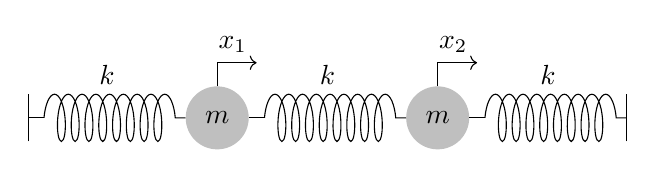
\begin{tikzpicture}
        % ばね (0,0) -- (2,0)
        \coordinate (left) at (0,0);
        \coordinate (right) at ($(left)+(2,0)$);
        \draw (left) -- ($(left)+(0.2,0)$); %左の棒
        \draw[decoration={coil,aspect=0.3,amplitude=0.3cm,segment length=1.75mm}] 
        decorate {($(left)+(0.2,0)$) -- (right)}; %本体
        \node [above=0.3cm] at ($(left)+(1,0)$) {$k$};

        % 左壁
        \draw ($(left)+(0,-0.3)$) -- ($(left)+(0,0.3)$);

        % 質点 (半径は0.4)
        \coordinate (center) at ($(right)+(0.4,0)$);
        \fill[lightgray] (center) circle (0.4);
        \node at (center) {$m$};
        % 座標 x_1
        \draw[->] ($(center)+(0,0.4)$) -- ($(center)+(0,0.7)$) -- ($(center)+(0.5,0.7)$) node [above left] {$x_1$};

        % ばね (2.8) -- (4.8)
        \coordinate (left) at (2.8,0);
        \coordinate (right) at ($(left)+(2,0)$);
        \draw (left) -- ($(left)+(0.2,0)$); %左の棒
        \draw[decoration={coil,aspect=0.3,amplitude=0.3cm,segment length=1.75mm}] 
        decorate {($(left)+(0.2,0)$) -- (right)}; %本体
        \node [above=0.3cm] at ($(left)+(1,0)$) {$k$};

        % 質点 (半径は0.4)
        \coordinate (center) at ($(right)+(0.4,0)$);
        \fill[lightgray] (center) circle (0.4);
        \node at (center) {$m$};
        % 座標 x_2
        \draw[->] ($(center)+(0,0.4)$) -- ($(center)+(0,0.7)$) -- ($(center)+(0.5,0.7)$) node [above left] {$x_2$};

        % ばね (5.6) -- (7.6)
        \coordinate (left) at (5.6,0);
        \coordinate (right) at ($(left)+(2,0)$);
        \draw (left) -- ($(left)+(0.2,0)$); %左の棒
        \draw[decoration={coil,aspect=0.3,amplitude=0.3cm,segment length=1.75mm}] 
        decorate {($(left)+(0.2,0)$) -- (right)}; %本体
        \node [above=0.3cm] at ($(left)+(1,0)$) {$k$};

        % 右壁
        \draw ($(right)+(0,-0.3)$) -- ($(right)+(0,0.3)$);

    \end{tikzpicture}
\end{center}

自由度2の連成振動の運動方程式は,
\begin{align}
    m \dv[2]{x_1}{t} &= -kx_1 + k(x_2 - x_1) \\
    m \dv[2]{x_2}{t} &= -kx_2 - k(x_2 - x_1)
\end{align}
である. $\vb*{v} = \qty(x_1, x_2)$ とすると, 上記の2つの運動方程式は行列を使って以下のように書ける.
\begin{equation}
    \label{eq:origin}
    m \dv[2]{\vb*{v}}{t}
    =
    \mqty[-2k & k \\ k & -2k] \vb*{v}
\end{equation}
\eqref{eq:origin} の右辺の行列は必ず対称行列になる (ToDo: 検討). 
これを, 座標を基準座標に取り替えることで独立な2つの振動に分解する. 基準座標に取り替るというのは, \eqref{eq:origin} の右辺の行列が対角行列になること. 対称行列は必ず対角化できる\footnote{\href{https://ja.wikipedia.org/wiki/\%E5\%AF\%BE\%E7\%A7\%B0\%E8\%A1\%8C\%E5\%88\%97}{wikipedia}を参照}. 

\end{document}